\chapter{API para módulos de matemáticos plugáveis} \label{cap:proposta}

Considerando as necessidades do ``Empurrando Juntos'', foram identificados requisitos funcionais e não funcionais 
da aplicação.

\section*{Requisitos Funcionais}

Uma avaliação do escopo da plataforma ``Empurrando Juntos'' permitiu o levantamento de características desejadas do sistema e,
consequentemente, alguns requisitos associados, que foram sumarizados na Tabela \ref{tab:requisitos}.

\begin{table}[h!]
\centering
\caption{Requisitos funcionais de alto nível da aplicação.}
\label{tab:requisitos}
\begin{tabular}{@{}cl@{}}
\toprule
\textbf{Característica}                      & \multicolumn{1}{c}{\textbf{Requisito}}                                                                                                \\ \midrule
\multirow{5}{*}{Gerenciamento de Usuário}    & O sistema deve permitir o cadastro de usuários                                                                                        \\
					    & O sistema deve permitir a alteração de usuários                                                                                       \\
					    & O sistema deve permitir a exclusão de usuários                                                                                         \\
					    & \begin{tabular}[c]{@{}l@{}}O sistema deve permitir a autenticação de usuários \\ cadastrados na plataforma\end{tabular}			\\
					    &  \begin{tabular}[c]{@{}l@{}}O sistema deve permitir a autenticação de usuários \\ cadastrados no Facebook\end{tabular}                     \\ \midrule
\multirow{3}{*}{Gerenciamento de Conversa}   & O sistema deve permitir o cadastro de conversas                                                                                       \\
					    & O sistema deve permitir a alteração de conversas                                                                                      \\
					    & O sistema deve permitir a exclusão de conversas                                                                                       \\ \midrule
\multirow{4}{*}{Gerenciamento de Comentário} & O sistema deve permitir o cadastro de comentários em conversas                                                                        \\
					    & O sistema deve permitir a alteração de comentários                                                                                    \\
					    & O sistema deve permitir a exclusão de comentários                                                                                     \\ 
					    & O sistema deve permitir que o usuário vote em comentários                                                                             \\ \midrule
Agrupamento de usuários                      & \begin{tabular}[c]{@{}l@{}}O sistema deve permitir a 
					      visualização dos usuários agrupados \\ de acordo com os votos dados\end{tabular} \\ \bottomrule
  \end{tabular}
    \end{table}
      
  
\section*{Requisitos não funcionais}		
    
Todos os serviços da API serão providos para a plataforma por meio de uma interface HTTP/HTTPS utilizando o estilo arquitetural REST.
A API deve possibilitar a escolha do módulo matemático a ser utilizado, considerando as opções previamente implementadas.

A autenticação e autorização das aplicações, e seus respectivos usuários devem ser realizadas por meio de \textit{tokens}.

A tecnologia definida para implementação da solução proposta foi a linguagem Python juntamente com os \textit{frameworks}
Django e Django Rest Framework, utilizando o banco de dados PostgreSQL.

Outro aspecto importante para esta aplicação é a questão da manutenibilidade, pois como será um software livre, a solução
deve ser desenvolvida de uma maneira que seja possível evoluir facilmente pela da comunidade.
Com isto em mente, foram definidos os seguintes padrões para o desenvolvimento da aplicação, considerando as tecnologias definidas:
utilização do PEP8 \footnotemark como folha de estilos e a utilização da especificação JSON API \footnotemark para formatação das respostas da API.
\footnotetext{Folha de estilos PEP8. Disponível em \href{https://www.python.org/dev/peps/pep-0008/}{https://www.python.org/dev/peps/pep-0008}.}
\footnotetext{Especificação JSON API. Disponível em \href{http://jsonapi.org/}{http://jsonapi.org}.}

\section{Arquitetura da solução}

Considerando o objetivo do trabalho de implementar uma API capaz de trabalhar com 
módulos matemáticos plugáveis, a solução proposta está representada na Figura \ref{fig:pentano}, 
na qual são indicados os dois tipos de módulos tratados na solução: API e \textit{Math} ou Matemático.
 
\begin{figure}[h!]
\centering
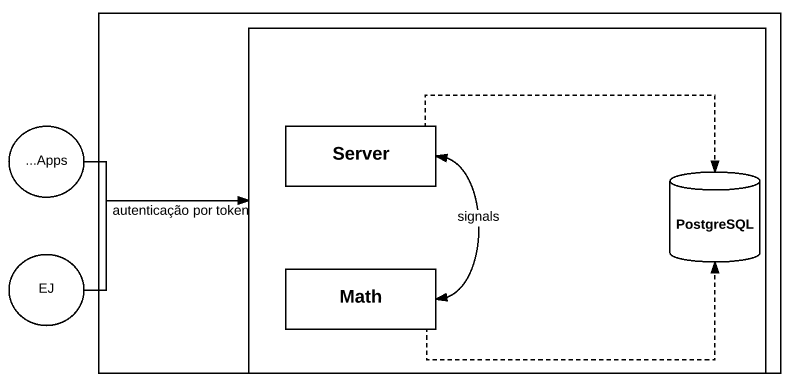
\includegraphics[scale=0.7]{figuras/esquema_pentano.png}
\caption{Estrutura do Pentano}
\label{fig:pentano}
\end{figure}

O módulo de API é responsável por gerenciar as conversas, comentários, votos
e cuidar de todos os aspectos da autenticação das aplicações. Os módulos \textit{Math} são responsáveis por realizar
a clusterização, criando os grupos com os respectivos usuários. 
A ideia é que esses módulos sejam outras aplicações que implementem a interface definida no protocolo. Ou seja, 
fica a cargo da implantação do sistema de associar a API desenvolvida neste trabalho com algum módulo matemático 
existente ou novo.

Para o módulo de API, foram mapeadas as entidades principais e os relacionamentos entre elas. 
As principais entidades que foram identificadas são Usuário, Conversa e Comentário. Um usuário pode criar
conversas e comentários para cada conversa e participar de outras conversas, criadas por outros usuários.
A participação de um usuário em uma conversa é dada pelo ato de criação de comentários naquela conversa ou
no ato de votar em um comentário de uma conversa. Esse mapeamento é ilustrado na Figura \ref{fig:entidades}.

\begin{figure}[h!]
\centering
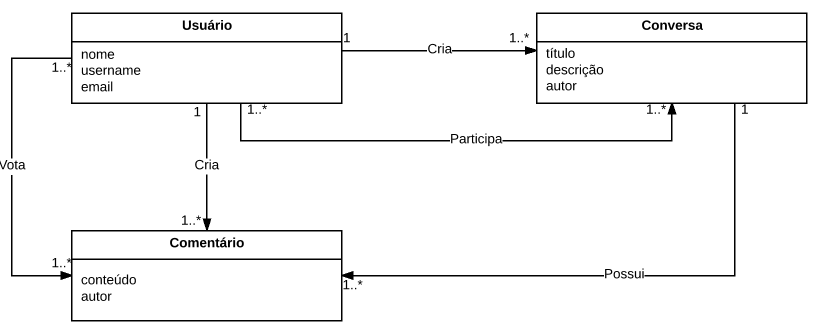
\includegraphics[scale=0.5]{figuras/entidades.png}
\caption{Relacionamento das principais entidades da API}
\label{fig:entidades}
\end{figure}

Como o \textit{framework} Django foi escolhido como tecnologia de implementação da API, a arquitetura proposta foi pensada valendo-se de 
recursos providos pelo própria arquitetura do \textit{framework}.
No Django, uma aplicação web é abstraída como um projeto, e um projeto é composto por uma coleção de aplicações
(ou, de forma abreviada, \textit{apps}) independentes, que
são pacotes Python que proveem um conjunto de funcionalidades relacionadas e podem ser reutilizados \cite{django_apps}.

Portanto, toda a solução foi componentizada utilizando \textit{apps} do 
Django. Considerando os requisitos funcionais e não funcionais da solução, especificados anteriormente, a arquitetura da solução foi definida 
conforme a Figura \ref{fig:arquitetura_api}, onde no módulo \textit{API} temos dois \textit{apps} independentes, um responsável
por cuidar de toda parte de autenticação da aplicação (\textit{app} de contas) e o outro para gerenciar as entidades apresentadas na
Figura \ref{fig:entidades} (\textit{app} de conversas). 

\begin{figure}[h!]
\centering
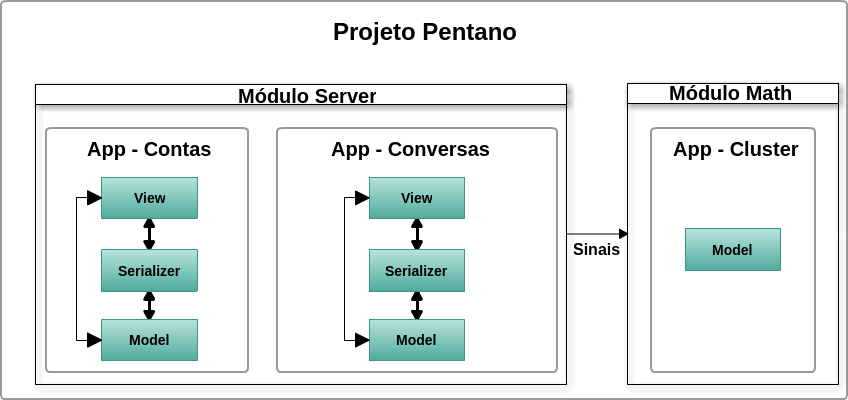
\includegraphics[scale=0.8]{figuras/arquitetura_api.png}
\caption{Entidades da API}
\label{fig:arquitetura_api}
\end{figure}

Para cada \textit{app} foi definida uma arquitetura
em 3 camadas: \textit{models}, \textit{views} e \textit{serializers}.
A camada \textit{view} recebe e responde as requisições provenientes do cliente.
A camada \textit{serializer} é responsável pelo tratamento e formatação dos dados das \textit{models}
para renderização em JSON, seguindo a especificação JSON API.
Por fim, a camada \textit{model} contém aspectos negociais relacionados a cada uma das entidades definidas na 
Figura \ref{fig:entidades}. 

\section{Protocolo de Comunicação}

Para a comunicação entre a API e o módulo matemático escolhido, foi desenvolvido um protocolo de comunicação com base
em uma plataforma de execução de tarefas assíncronas, o Celery \footnotemark. 
Essa ferramenta em conjunto com a interface definida e um \textit{message broker}, que é uma plataforma intermediária
entre duas aplicações para troca de mensagens, formam a comunicação entre a API e o módulo responsável pela clusterização. 
Uma visão geral do protocolo pode ser vista na 
Figura \ref{fig:protocolo}.
\footnotetext{http://www.celeryproject.org/}

\begin{figure}[bt!]
\centering
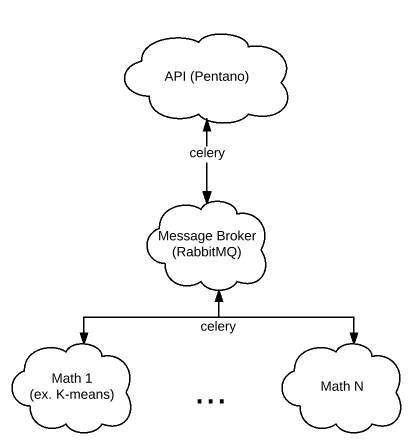
\includegraphics[scale=0.6]{figuras/protocolo.png}
\caption{Protocolo de comunicação entre os módulos - API e \textit{Math}}
\label{fig:protocolo}
\end{figure}

Para estabelecer comunicação com a API, o módulo matemático deve seguir as seguintes diretrizes:
\begin{itemize}
  \item Deve ser uma aplicação que execute o Celery em um de seus apps;
  \item Deve possuir um arquivo de \textit{tasks}, no qual devem constar as tarefas a serem executadas na aplicação pelo Celery;
  \item Deve implementar as 4 tarefas especificadas na Tabela \ref{tab:tasks};
  \item Deve implementar as entidades e os atributos especificados na Tabela \ref{tab:entidades_math}.
\end{itemize}

\begin{table}[]
\centering
\caption{Tarefas dos módulos matemáticos}
\label{tab:tasks}
\begin{tabular}{@{}lll@{}}
\multicolumn{1}{c}{\textbf{Tarefa}}                                                & \multicolumn{1}{c}{\textbf{Parâmetros}}                                                                               & \multicolumn{1}{c}{\textbf{Retorno}} \\ \midrule
\begin{tabular}[c]{@{}l@{}}Adicionar nova conversa \\ (pentano.new\_conversation)\end{tabular} & Identificador da conversa                                                                                             & Confirmação de Sucesso               \\ \midrule
\begin{tabular}[c]{@{}l@{}}Adicionar novo comentário \\ (pentano.add\_comment)\end{tabular}    & \begin{tabular}[c]{@{}l@{}}Identificador da conversa\\ Identificador do comentário\\ Texto do comentário\end{tabular} & Confirmação de Sucesso               \\ \midrule
\begin{tabular}[c]{@{}l@{}}Adicionar novo voto\\ (pentano.add\_votes)\end{tabular}             & \begin{tabular}[c]{@{}l@{}}Identificador da conversa\\ DataFrame com o usuário e o voto\end{tabular}                                             & Confirmação de Sucesso               \\ \midrule
\begin{tabular}[c]{@{}l@{}}Clusterizar\\ (pentano.get\_cluster)\end{tabular}                   & \begin{tabular}[c]{@{}l@{}}Identificador da conversa\\ Identificadores dos usuários amigos\end{tabular}               & Grupos de usuários (clusters)        \\ \bottomrule
\end{tabular}
\end{table}

\begin{table}[]
\centering
\caption{Entidades e atributos dos módulos matemáticos}
\label{tab:entidades_math}
\begin{tabular}{@{}ll@{}}
\toprule
\multicolumn{1}{c}{\textbf{Entidade}} & \multicolumn{1}{c}{\textbf{Atributos}} \\ \midrule
Usuário                               & Identificador                          \\
Conversa                              & Identificador                          \\
Comentário                            & Identificador                          \\
Voto                                  & Valor                                  \\ \bottomrule
\end{tabular}
\end{table}

Considerando que o módulo matemático implemente todas as diretrizes definidas acima, a comunicação é realizada com 
os seguintes passos:
  
\begin{enumerate}
 \item O cliente realiza uma das requisições relacionada a uma das 4 tarefas da Tabela \ref{tab:tasks};
 \item A API processa a requisição e faz a chamada da tarefa para o \textit{message broker};
 \item O Celery executando no projeto onde encontra-se o módulo matemático captura a chamada da tarefa através do mesmo \textit{message broker} e 
 executa a tarefa especificada;
 \item O módulo matemático retorna o resultado de execução da tarefa;
 \item A API recebe o resultado retornado do módulo matemático, identificando o sucesso ou a falha da tarefa executada.
\end{enumerate}

\vfill
\pagebreak
\begin{figure}[bt!]
\centering
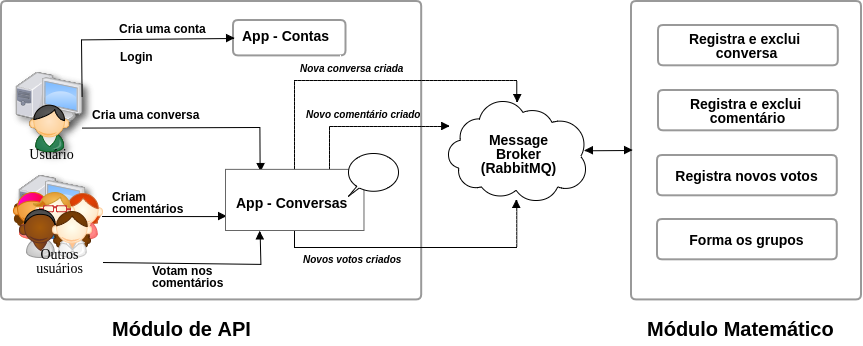
\includegraphics[scale=0.6]{figuras/resumo_ej_api.png}
\caption{Funcionamento do Empurrando Juntos - Comunicação entre os módulos}
\label{fig:resumo_ej_api}
\end{figure}


Na Figura \ref{fig:resumo_ej_api} é apresentado o fluxo de funcionamento do Empurrando Juntos de acordo com a arquitetura
estabelecida e a API desenvolvida. Inicialmente, um usuário faz o cadastro e/ou autentica na aplicação, cuja requisição é tratada pelo \textit{app} de contas.
Após a autenticação do usuário, ele pode criar conversas e comentários na aplicação. Outros usuários podem criar comentários e votar
nos comentários. Todas essas operações relacionadas à conversas, comentários e votos são tratadas pelo \textit{app} de conversas.
Quando uma nova conversa é criada, um novo comentário ou um novo voto é realizado em algum comentário de uma conversa, o 
\textit{app} de conversas faz uma chamada para a tarefa correspondente. Essa chamada é recebida pelo módulo que realiza a clusterização, 
com base no Celery e no textit{message broker}. Quando o número de votos configurado no sistema é atingido o \textit{app} de conversas
faz uma chamada para a tarefa de clusterização que ao ser recebida pelo módulo matemático, é a tarefa responsável por calcular
os \textit{clusters} considerando o usuário do novo voto, gerando novos grupos de usuários.